\documentclass[11pt,preprint]{elsarticle}

\usepackage{lmodern}
%%%% My spacing
\usepackage{setspace}
\setstretch{1.2}
\DeclareMathSizes{12}{14}{10}{10}

% Wrap around which gives all figures included the [H] command, or places it "here". This can be tedious to code in Rmarkdown.
\usepackage{float}
\let\origfigure\figure
\let\endorigfigure\endfigure
\renewenvironment{figure}[1][2] {
    \expandafter\origfigure\expandafter[H]
} {
    \endorigfigure
}

\let\origtable\table
\let\endorigtable\endtable
\renewenvironment{table}[1][2] {
    \expandafter\origtable\expandafter[H]
} {
    \endorigtable
}


\usepackage{ifxetex,ifluatex}
\usepackage{fixltx2e} % provides \textsubscript
\ifnum 0\ifxetex 1\fi\ifluatex 1\fi=0 % if pdftex
  \usepackage[T1]{fontenc}
  \usepackage[utf8]{inputenc}
\else % if luatex or xelatex
  \ifxetex
    \usepackage{mathspec}
    \usepackage{xltxtra,xunicode}
  \else
    \usepackage{fontspec}
  \fi
  \defaultfontfeatures{Mapping=tex-text,Scale=MatchLowercase}
  \newcommand{\euro}{€}
\fi

\usepackage{amssymb, amsmath, amsthm, amsfonts}

\def\bibsection{\section*{References}} %%% Make "References" appear before bibliography


\usepackage[numbers]{natbib}

\usepackage{longtable}
\usepackage[margin=2.3cm,bottom=2cm,top=2.5cm, includefoot]{geometry}
\usepackage{fancyhdr}
\usepackage[bottom, hang, flushmargin]{footmisc}
\usepackage{graphicx}
\numberwithin{equation}{section}
\numberwithin{figure}{section}
\numberwithin{table}{section}
\setlength{\parindent}{0cm}
\setlength{\parskip}{1.3ex plus 0.5ex minus 0.3ex}
\usepackage{textcomp}
\renewcommand{\headrulewidth}{0.2pt}
\renewcommand{\footrulewidth}{0.3pt}

\usepackage{array}
\newcolumntype{x}[1]{>{\centering\arraybackslash\hspace{0pt}}p{#1}}

%%%%  Remove the "preprint submitted to" part. Don't worry about this either, it just looks better without it:
\makeatletter
\def\ps@pprintTitle{%
  \let\@oddhead\@empty
  \let\@evenhead\@empty
  \let\@oddfoot\@empty
  \let\@evenfoot\@oddfoot
}
\makeatother

 \def\tightlist{} % This allows for subbullets!

\usepackage{hyperref}
\hypersetup{breaklinks=true,
            bookmarks=true,
            colorlinks=true,
            citecolor=blue,
            urlcolor=blue,
            linkcolor=blue,
            pdfborder={0 0 0}}


% The following packages allow huxtable to work:
\usepackage{siunitx}
\usepackage{multirow}
\usepackage{hhline}
\usepackage{calc}
\usepackage{tabularx}
\usepackage{booktabs}
\usepackage{caption}


\newenvironment{columns}[1][]{}{}

\newenvironment{column}[1]{\begin{minipage}{#1}\ignorespaces}{%
\end{minipage}
\ifhmode\unskip\fi
\aftergroup\useignorespacesandallpars}

\def\useignorespacesandallpars#1\ignorespaces\fi{%
#1\fi\ignorespacesandallpars}

\makeatletter
\def\ignorespacesandallpars{%
  \@ifnextchar\par
    {\expandafter\ignorespacesandallpars\@gobble}%
    {}%
}
\makeatother


% definitions for citeproc citations
\NewDocumentCommand\citeproctext{}{}
\NewDocumentCommand\citeproc{mm}{%
\href{\#cite.\detokenize{#1}}{#2}\nocite{#1}}

\makeatletter
% allow citations to break across lines
\let\@cite@ofmt\@firstofone
% avoid brackets around text for \cite:
\def\@biblabel#1{}
\def\@cite#1#2{{#1\if@tempswa , #2\fi}}
\makeatother
\newlength{\cslhangindent}
\setlength{\cslhangindent}{1.5em}
\newlength{\csllabelwidth}
\setlength{\csllabelwidth}{3em}
\newenvironment{CSLReferences}[2] % #1 hanging-indent, #2 entry-spacing
{\begin{list}{}{%
	\setlength{\itemindent}{0pt}
	\setlength{\leftmargin}{0pt}
	\setlength{\parsep}{0pt}
	% turn on hanging indent if param 1 is 1
	\ifodd #1
	\setlength{\leftmargin}{\cslhangindent}
	\setlength{\itemindent}{-1\cslhangindent}
	\fi
	% set entry spacing
	\setlength{\itemsep}{#2\baselineskip}}}
{\end{list}}

\usepackage{calc}
\newcommand{\CSLBlock}[1]{\hfill\break\parbox[t]{\linewidth}{\strut\ignorespaces#1\strut}}
\newcommand{\CSLLeftMargin}[1]{\parbox[t]{\csllabelwidth}{\strut#1\strut}}
\newcommand{\CSLRightInline}[1]{\parbox[t]{\linewidth - \csllabelwidth}{\strut#1\strut}}
\newcommand{\CSLIndent}[1]{\hspace{\cslhangindent}#1}


\urlstyle{same}  % don't use monospace font for urls
\setlength{\parindent}{0pt}
\setlength{\parskip}{6pt plus 2pt minus 1pt}
\setlength{\emergencystretch}{3em}  % prevent overfull lines
\setcounter{secnumdepth}{5}

%%% Use protect on footnotes to avoid problems with footnotes in titles
\let\rmarkdownfootnote\footnote%
\def\footnote{\protect\rmarkdownfootnote}
\IfFileExists{upquote.sty}{\usepackage{upquote}}{}

%%% Include extra packages specified by user
\usepackage{booktabs}
\usepackage{longtable}
\usepackage{array}
\usepackage{multirow}
\usepackage{wrapfig}
\usepackage{float}
\usepackage{colortbl}
\usepackage{pdflscape}
\usepackage{tabu}
\usepackage{threeparttable}
\usepackage{threeparttablex}
\usepackage[normalem]{ulem}
\usepackage{makecell}
\usepackage{xcolor}

%%% Hard setting column skips for reports - this ensures greater consistency and control over the length settings in the document.
%% page layout
%% paragraphs
\setlength{\baselineskip}{12pt plus 0pt minus 0pt}
\setlength{\parskip}{12pt plus 0pt minus 0pt}
\setlength{\parindent}{0pt plus 0pt minus 0pt}
%% floats
\setlength{\floatsep}{12pt plus 0 pt minus 0pt}
\setlength{\textfloatsep}{20pt plus 0pt minus 0pt}
\setlength{\intextsep}{14pt plus 0pt minus 0pt}
\setlength{\dbltextfloatsep}{20pt plus 0pt minus 0pt}
\setlength{\dblfloatsep}{14pt plus 0pt minus 0pt}
%% maths
\setlength{\abovedisplayskip}{12pt plus 0pt minus 0pt}
\setlength{\belowdisplayskip}{12pt plus 0pt minus 0pt}
%% lists
\setlength{\topsep}{10pt plus 0pt minus 0pt}
\setlength{\partopsep}{3pt plus 0pt minus 0pt}
\setlength{\itemsep}{5pt plus 0pt minus 0pt}
\setlength{\labelsep}{8mm plus 0mm minus 0mm}
\setlength{\parsep}{\the\parskip}
\setlength{\listparindent}{\the\parindent}
%% verbatim
\setlength{\fboxsep}{5pt plus 0pt minus 0pt}



\begin{document}



\begin{frontmatter}  %

\title{SA Index Comparison}

% Set to FALSE if wanting to remove title (for submission)




\author[Add1]{Martin Raubenheimer 24954578}
\ead{martinraubs@gmail.com}





\address[Add1]{Department of Economics, Stellenbosch University, South
Africa}


\begin{abstract}
\small{
Abstract to be written here. The abstract should not be too long and
should provide the reader with a good understanding what you are writing
about. Academic papers are not like novels where you keep the reader in
suspense. To be effective in getting others to read your paper, be as
open and concise about your findings here as possible. Ideally, upon
reading your abstract, the reader should feel he / she must read your
paper in entirety.
}
\end{abstract}

\vspace{1cm}





\vspace{0.5cm}

\end{frontmatter}

\setcounter{footnote}{0}



%________________________
% Header and Footers
%%%%%%%%%%%%%%%%%%%%%%%%%%%%%%%%%
\pagestyle{fancy}
\chead{}
\rhead{}
\lfoot{}
\rfoot{\footnotesize Page \thepage}
\lhead{}
%\rfoot{\footnotesize Page \thepage } % "e.g. Page 2"
\cfoot{}

%\setlength\headheight{30pt}
%%%%%%%%%%%%%%%%%%%%%%%%%%%%%%%%%
%________________________

\headsep 35pt % So that header does not go over title




Introduction: data, how the indexes are built (lagged month-end weights,
fixed within the month). Composition: sector area charts and the
concentration table. Risk: GJR-GARCH plots (with a sentence on the IC
table), sector vol heatmap, constituent vol. Return: rolling return
plots, summary table, regime table. Active share: the chart and what it
implies for investors. Conclusion: one paragraph tying size, sector mix,
concentration, vol and return together.

\section{\texorpdfstring{Introduction
\label{Introduction}}{Introduction }}\label{introduction}

This report does a brief comparison the concentration, risk exposures ,
volatility, returns and active share between JSE indexes. Specifically
the CappedSWIX (which is the benchmark), LargeCaps, MidCaps and
SmallCaps.

\section{Index 'Composition}\label{index-composition}

The graph belows shows the different sector exposures of the indexes
over time: CappedSWIX: Its largest exposure has been industrials since
the beginning of the sample. Since 2017 resources has been occupying an
increasing share in the index. LargeCaps: Resources has been decreasing
and financials increasing. MidCaps:Already much more variation overtime
than the above. Resources adn financials are increasing its share where
industrials have largely declined. SmallCaps: Unclassified share has
decreased. Has by far the highest exposure to properties of all the
Indexes. Share of industrials has been increasing.

\begin{center}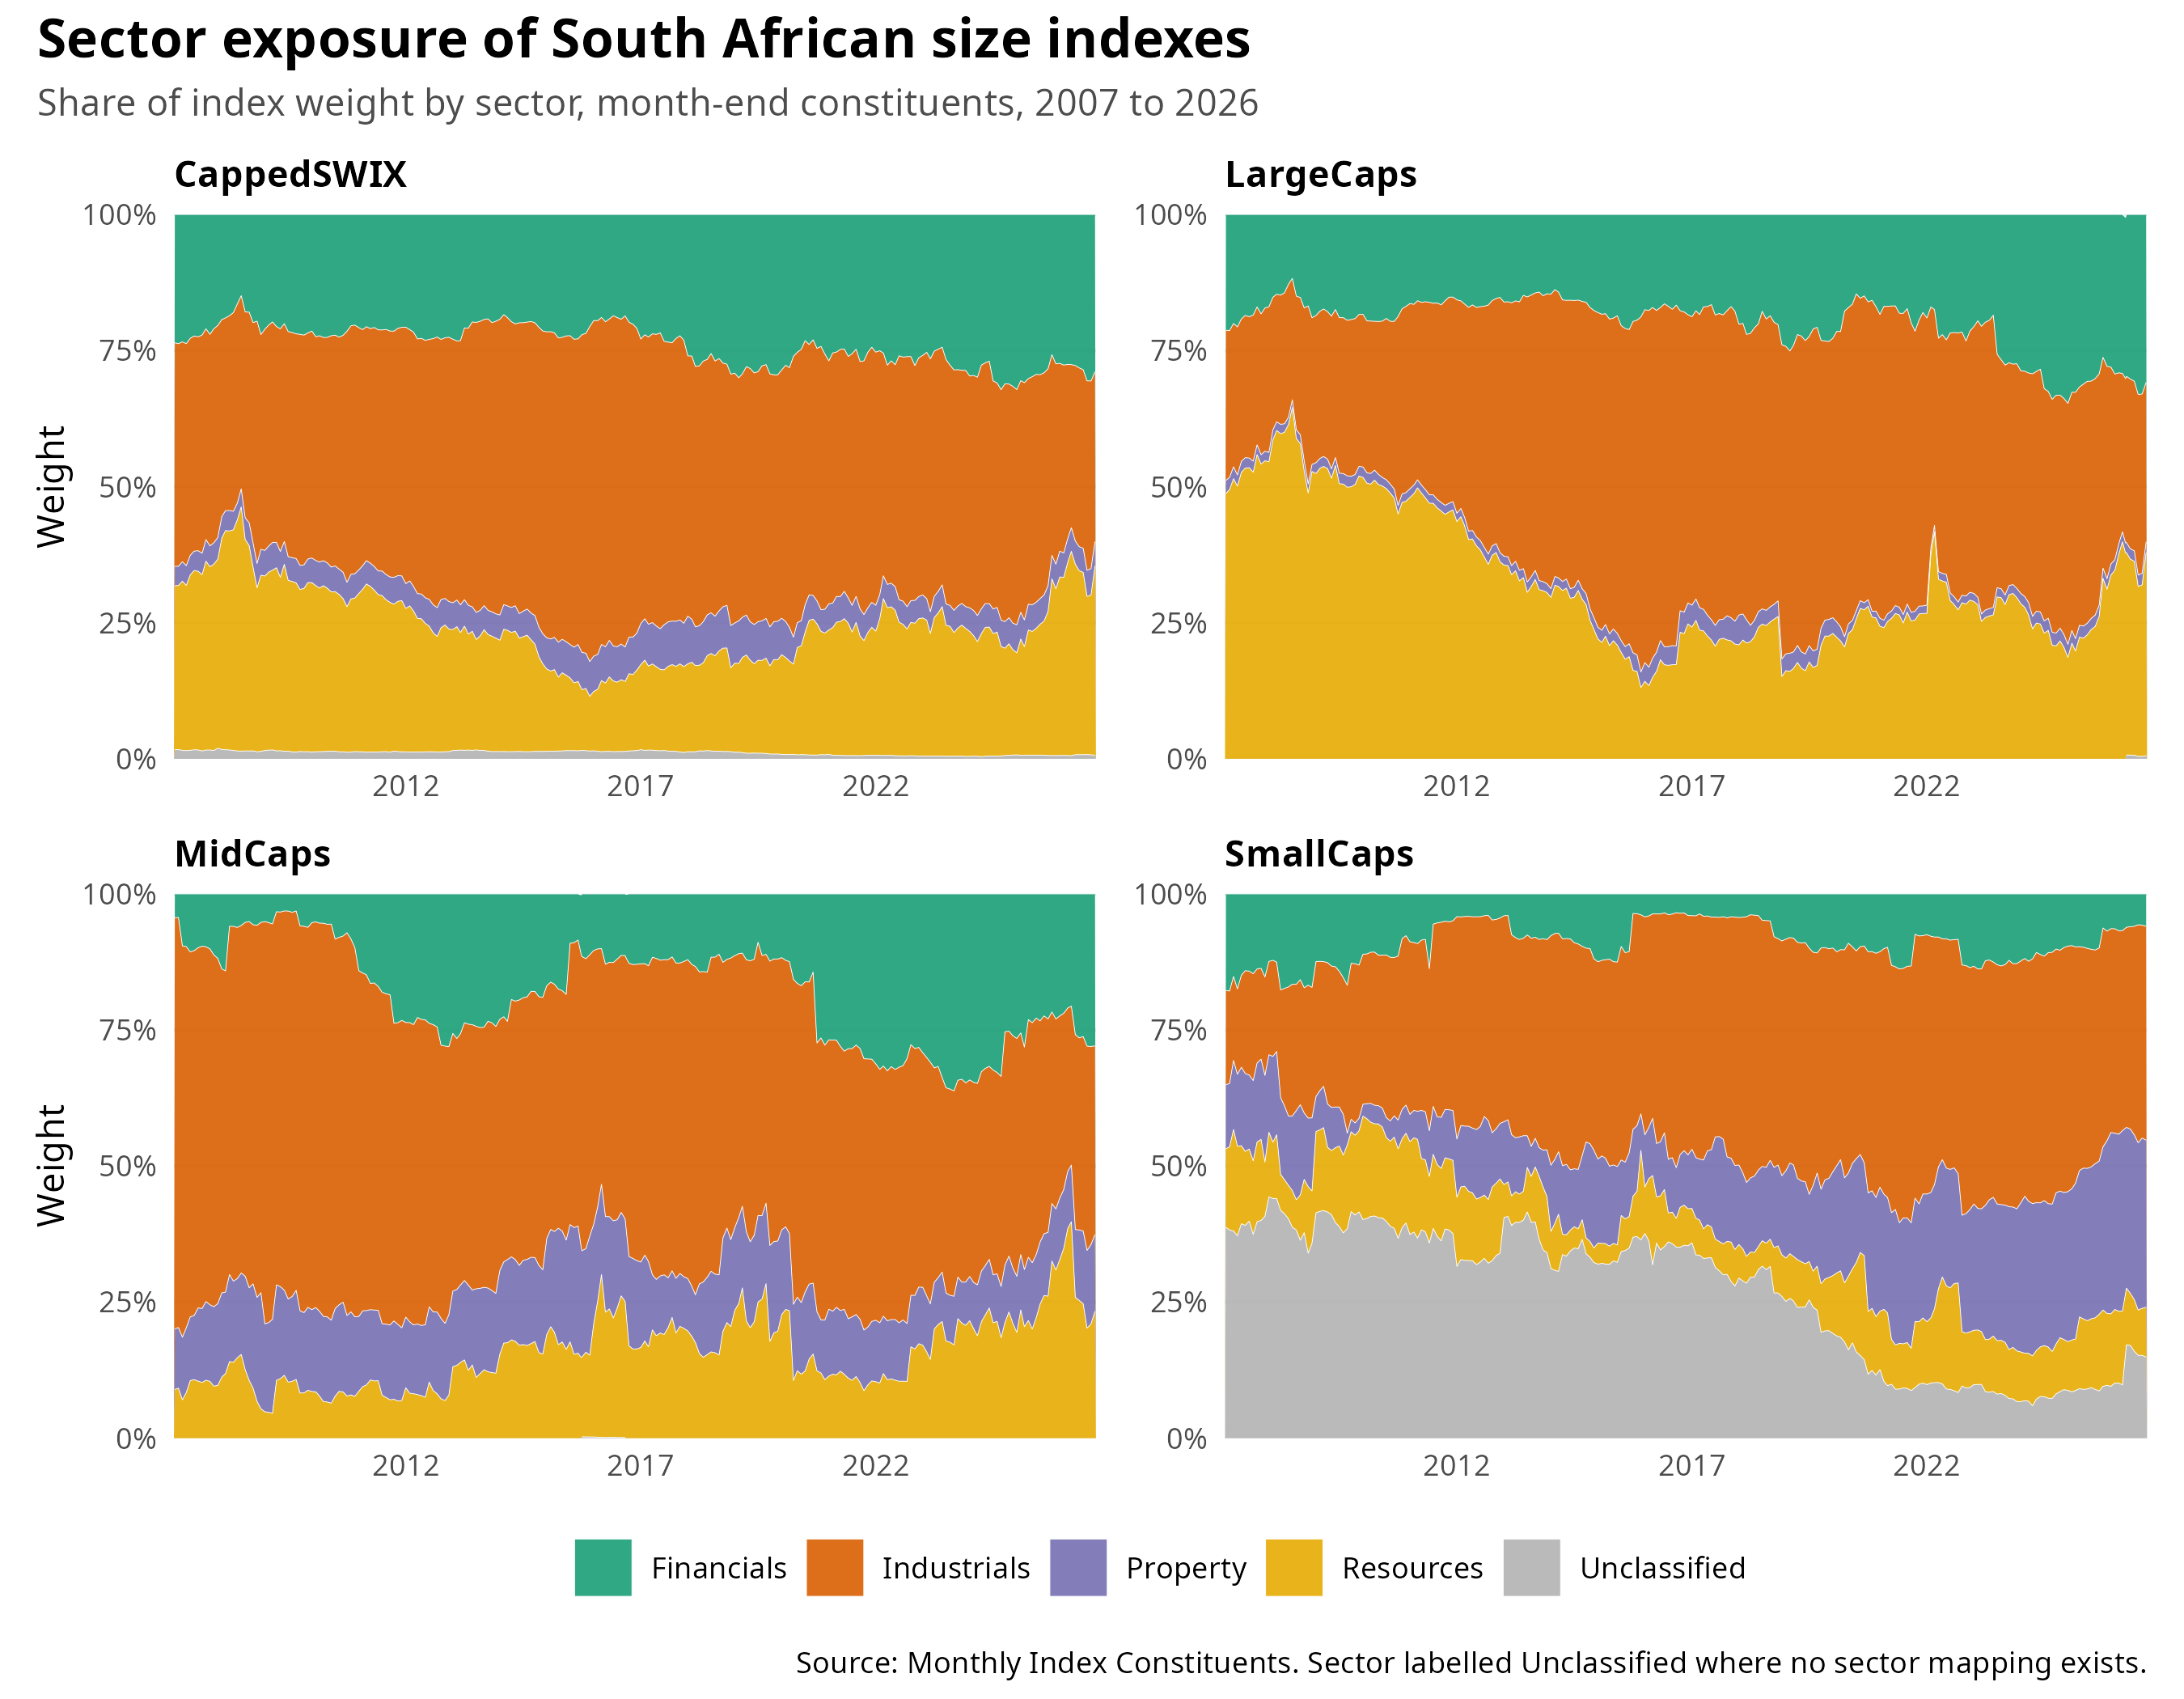
\includegraphics[width=1\linewidth]{../../figures/sector_exposure} \end{center}

The Herfindahl-Hirschman Index (HHI) measures portfolio concentration by
summing the squared weights of all holdings (\(\sum w_i^2\)), heavily
penalizing large, dominant positions. Taking its inverse (1/HHI) reveals
the effective number of stocks, showing how many equal-weighted holdings
an index truly behaves like.

\begin{center}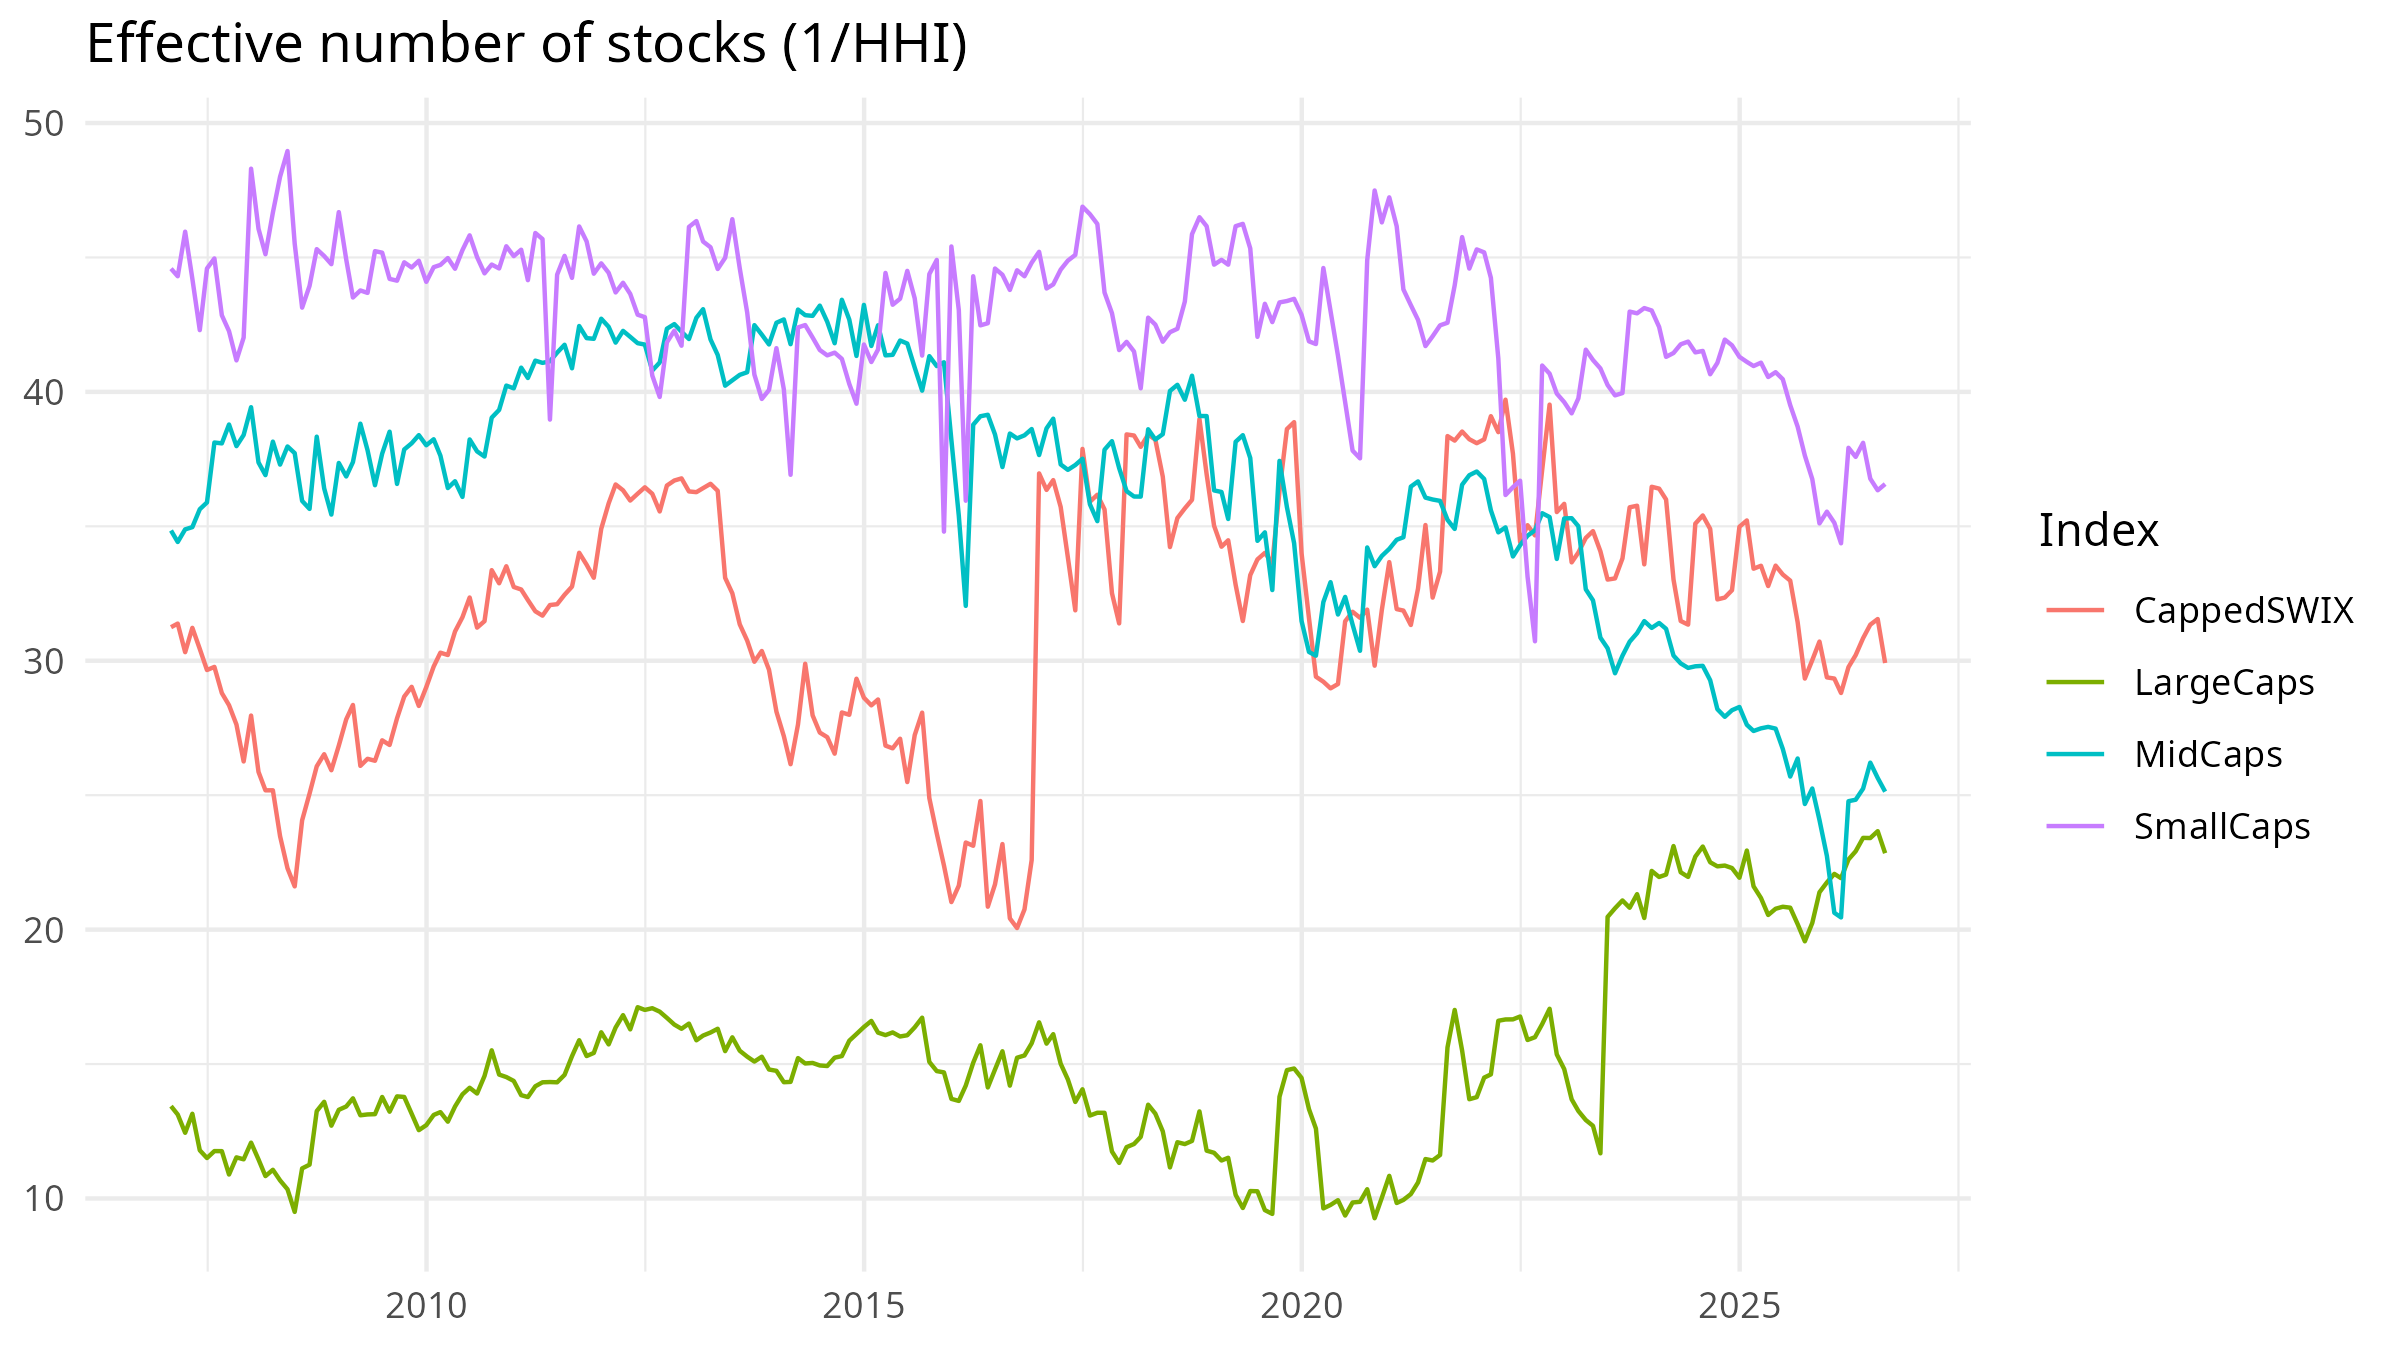
\includegraphics[width=1\linewidth]{../../figures/concentration} \end{center}

\begin{itemize}
\tightlist
\item
  CappedSWIX (red): Rebounded sharply in 2017 from severe concentration
  lows (\textasciitilde20 effective stocks) to stabilize between 30 and
  40. This shift reflects the JSE's introduction of a 10\% single-stock
  capping limit at quarterly rebalances, which curbed the outsized
  dominance of mega-caps like Naspers by redistributing excess weight
  across smaller constituents.
\item
  LargeCaps (green): Historically exhibit the highest concentration
  (hovering between 10 and 17 effective stocks), before experiencing a
  notable structural improvement in diversification after 2022 to sit
  above 20.
\item
  MidCaps (teal): Have steadily grown more concentrated over the past
  decade, declining from highs above 40 effective stocks toward the
  mid-20s.
\item
  SmallCaps (purple): Consistently remain the most diversified index,
  fluctuating between 35 and 49 effective stocks, though trending
  slightly lower in recent years. \newpage The table below show the
  average concentration, effective number of stocks and the weight of
  the top 5 and 10 stocks in each index.
\end{itemize}

\begin{longtable}[]{@{}lrrrr@{}}
\caption{Average concentration by index}\tabularnewline
\toprule\noalign{}
Index & N & EffN & Top5 & Top10 \\
\midrule\noalign{}
\endfirsthead
\toprule\noalign{}
Index & N & EffN & Top5 & Top10 \\
\midrule\noalign{}
\endhead
\bottomrule\noalign{}
\endlastfoot
CappedSWIX & 148.29 & 31.65 & 0.31 & 0.46 \\
LargeCaps & 39.75 & 15.08 & 0.48 & 0.66 \\
MidCaps & 53.25 & 36.31 & 0.24 & 0.41 \\
SmallCaps & 59.30 & 42.72 & 0.20 & 0.35 \\
\end{longtable}

\section{Index Risk Profile}\label{index-risk-profile}

GARCH models offer noise reduced volatility estimates. The GARCH model
family has models tremendously and the results of different can be found
in the appendix. The graph below shows the volatility from an eGARCH
model. Interestingly the results show that SmallCaps have less
``structure'' in their volatility meaning they are just extra noisy as
the most volatility. These stocks often dont trade much so some trades
can cause significant price changes.

\begin{center}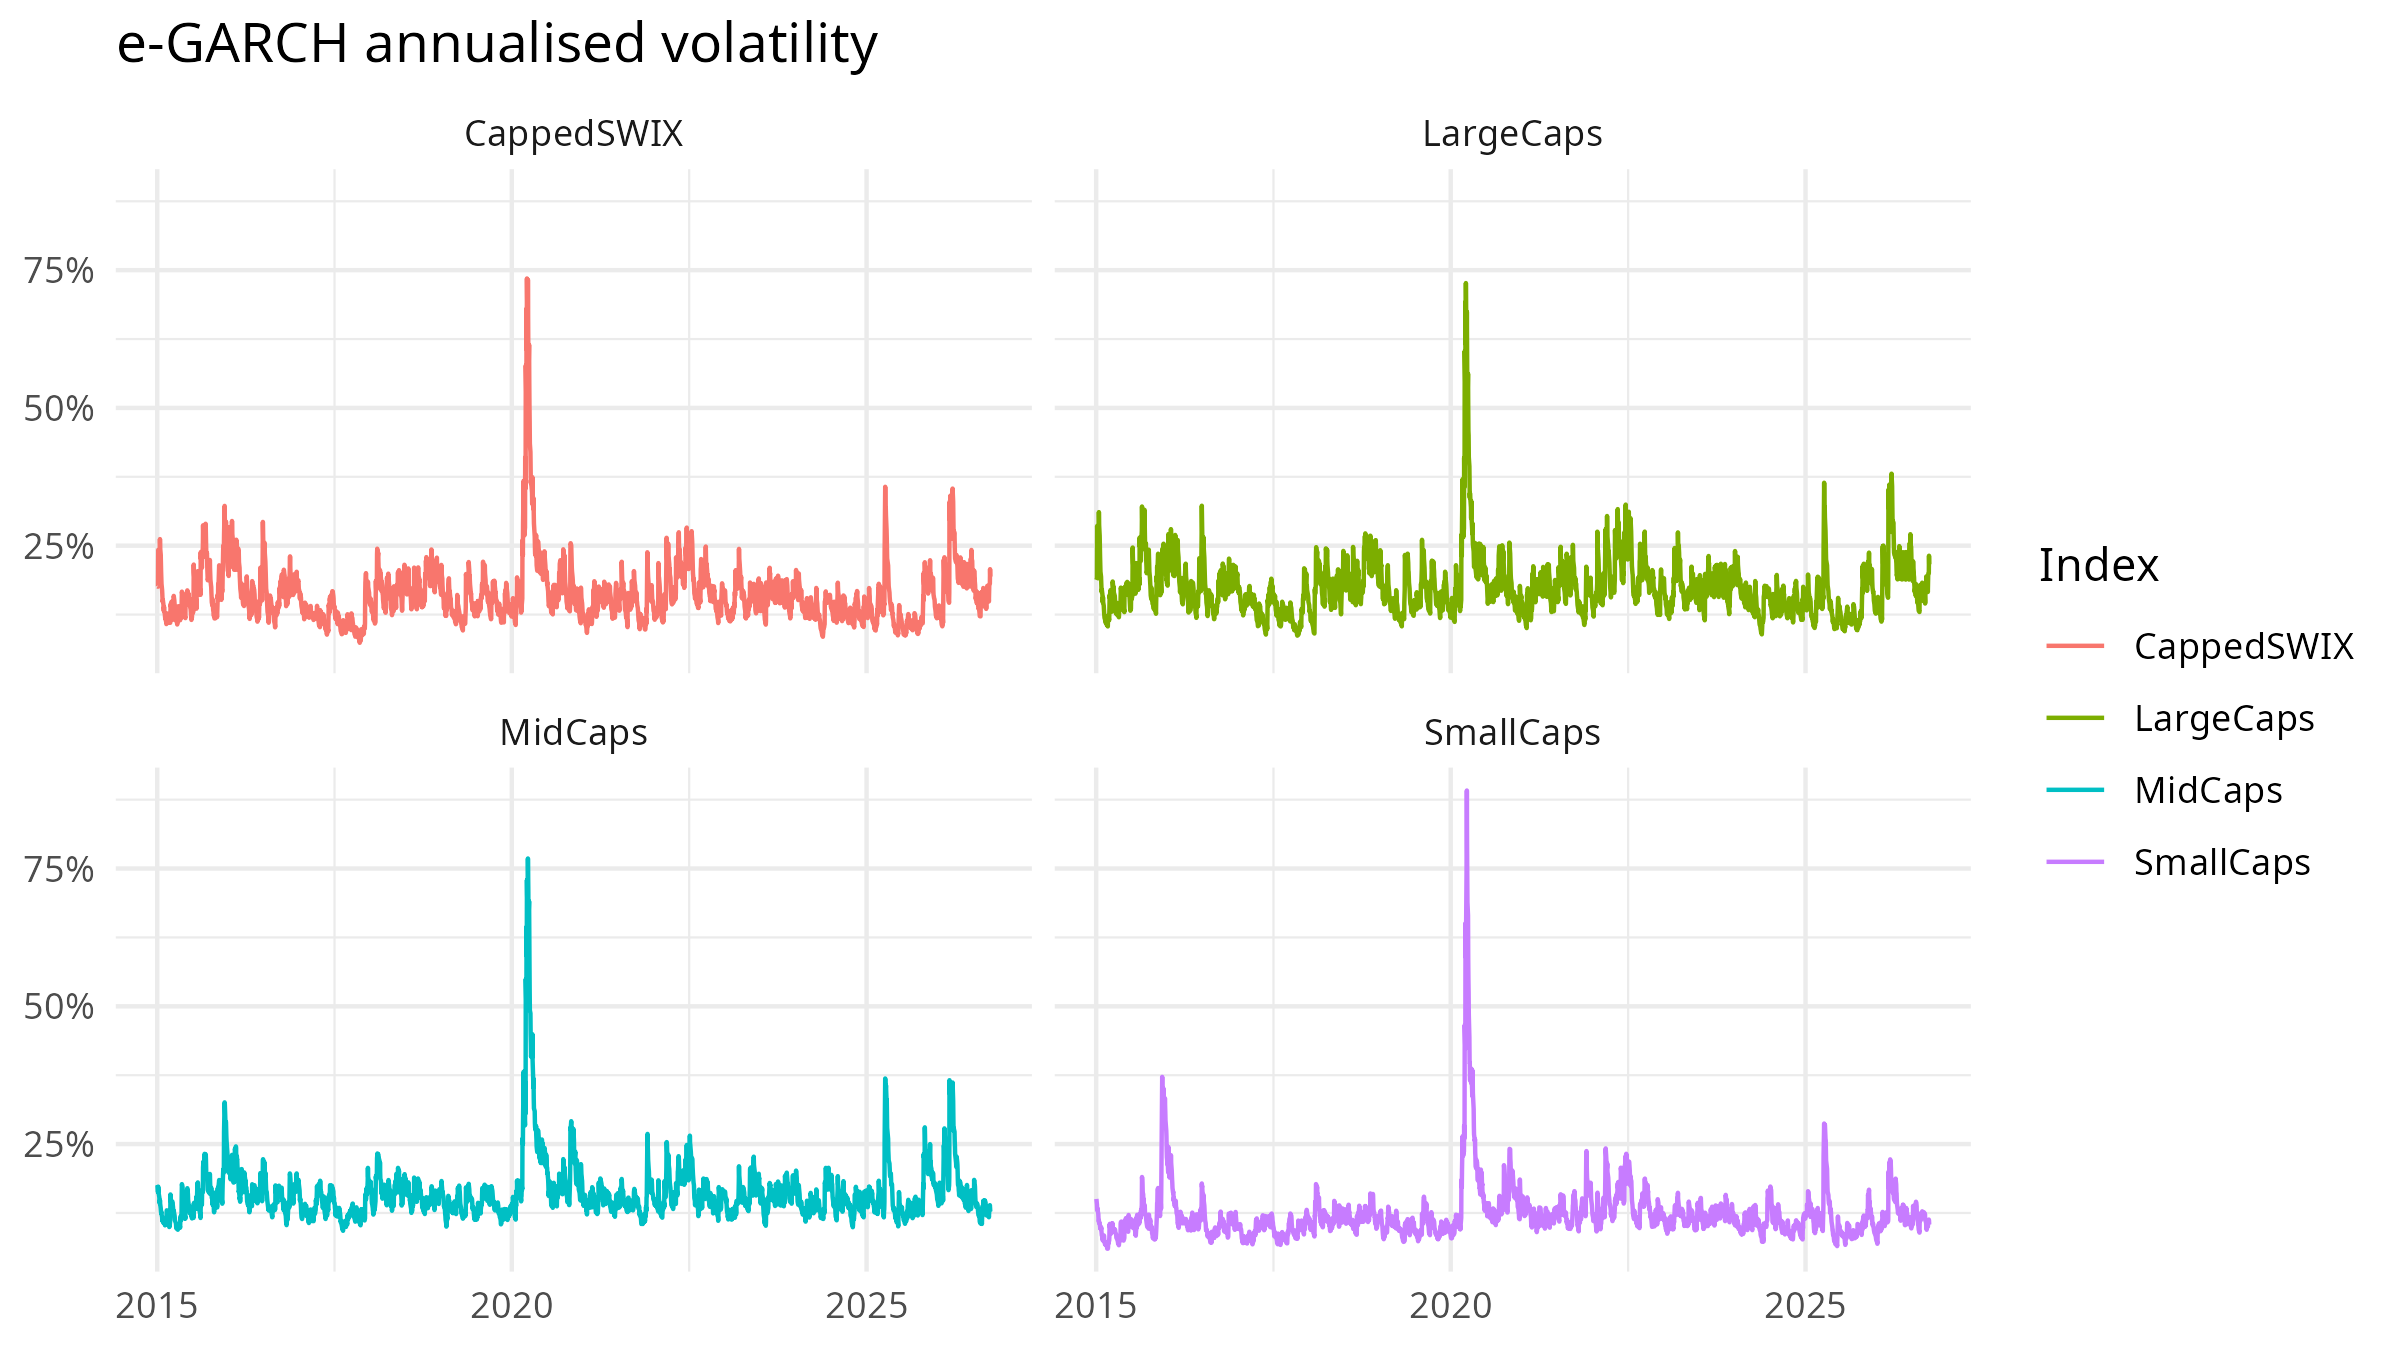
\includegraphics[width=1\linewidth]{../../figures/eGARCH_vol} \end{center}

In the graph below the median constituent volatility is plotted for each
index on a rolling 60-day basis. As to be expected SmallCaps have higher
volatility than the other indexes and LargeCaps having the least.

\begin{center}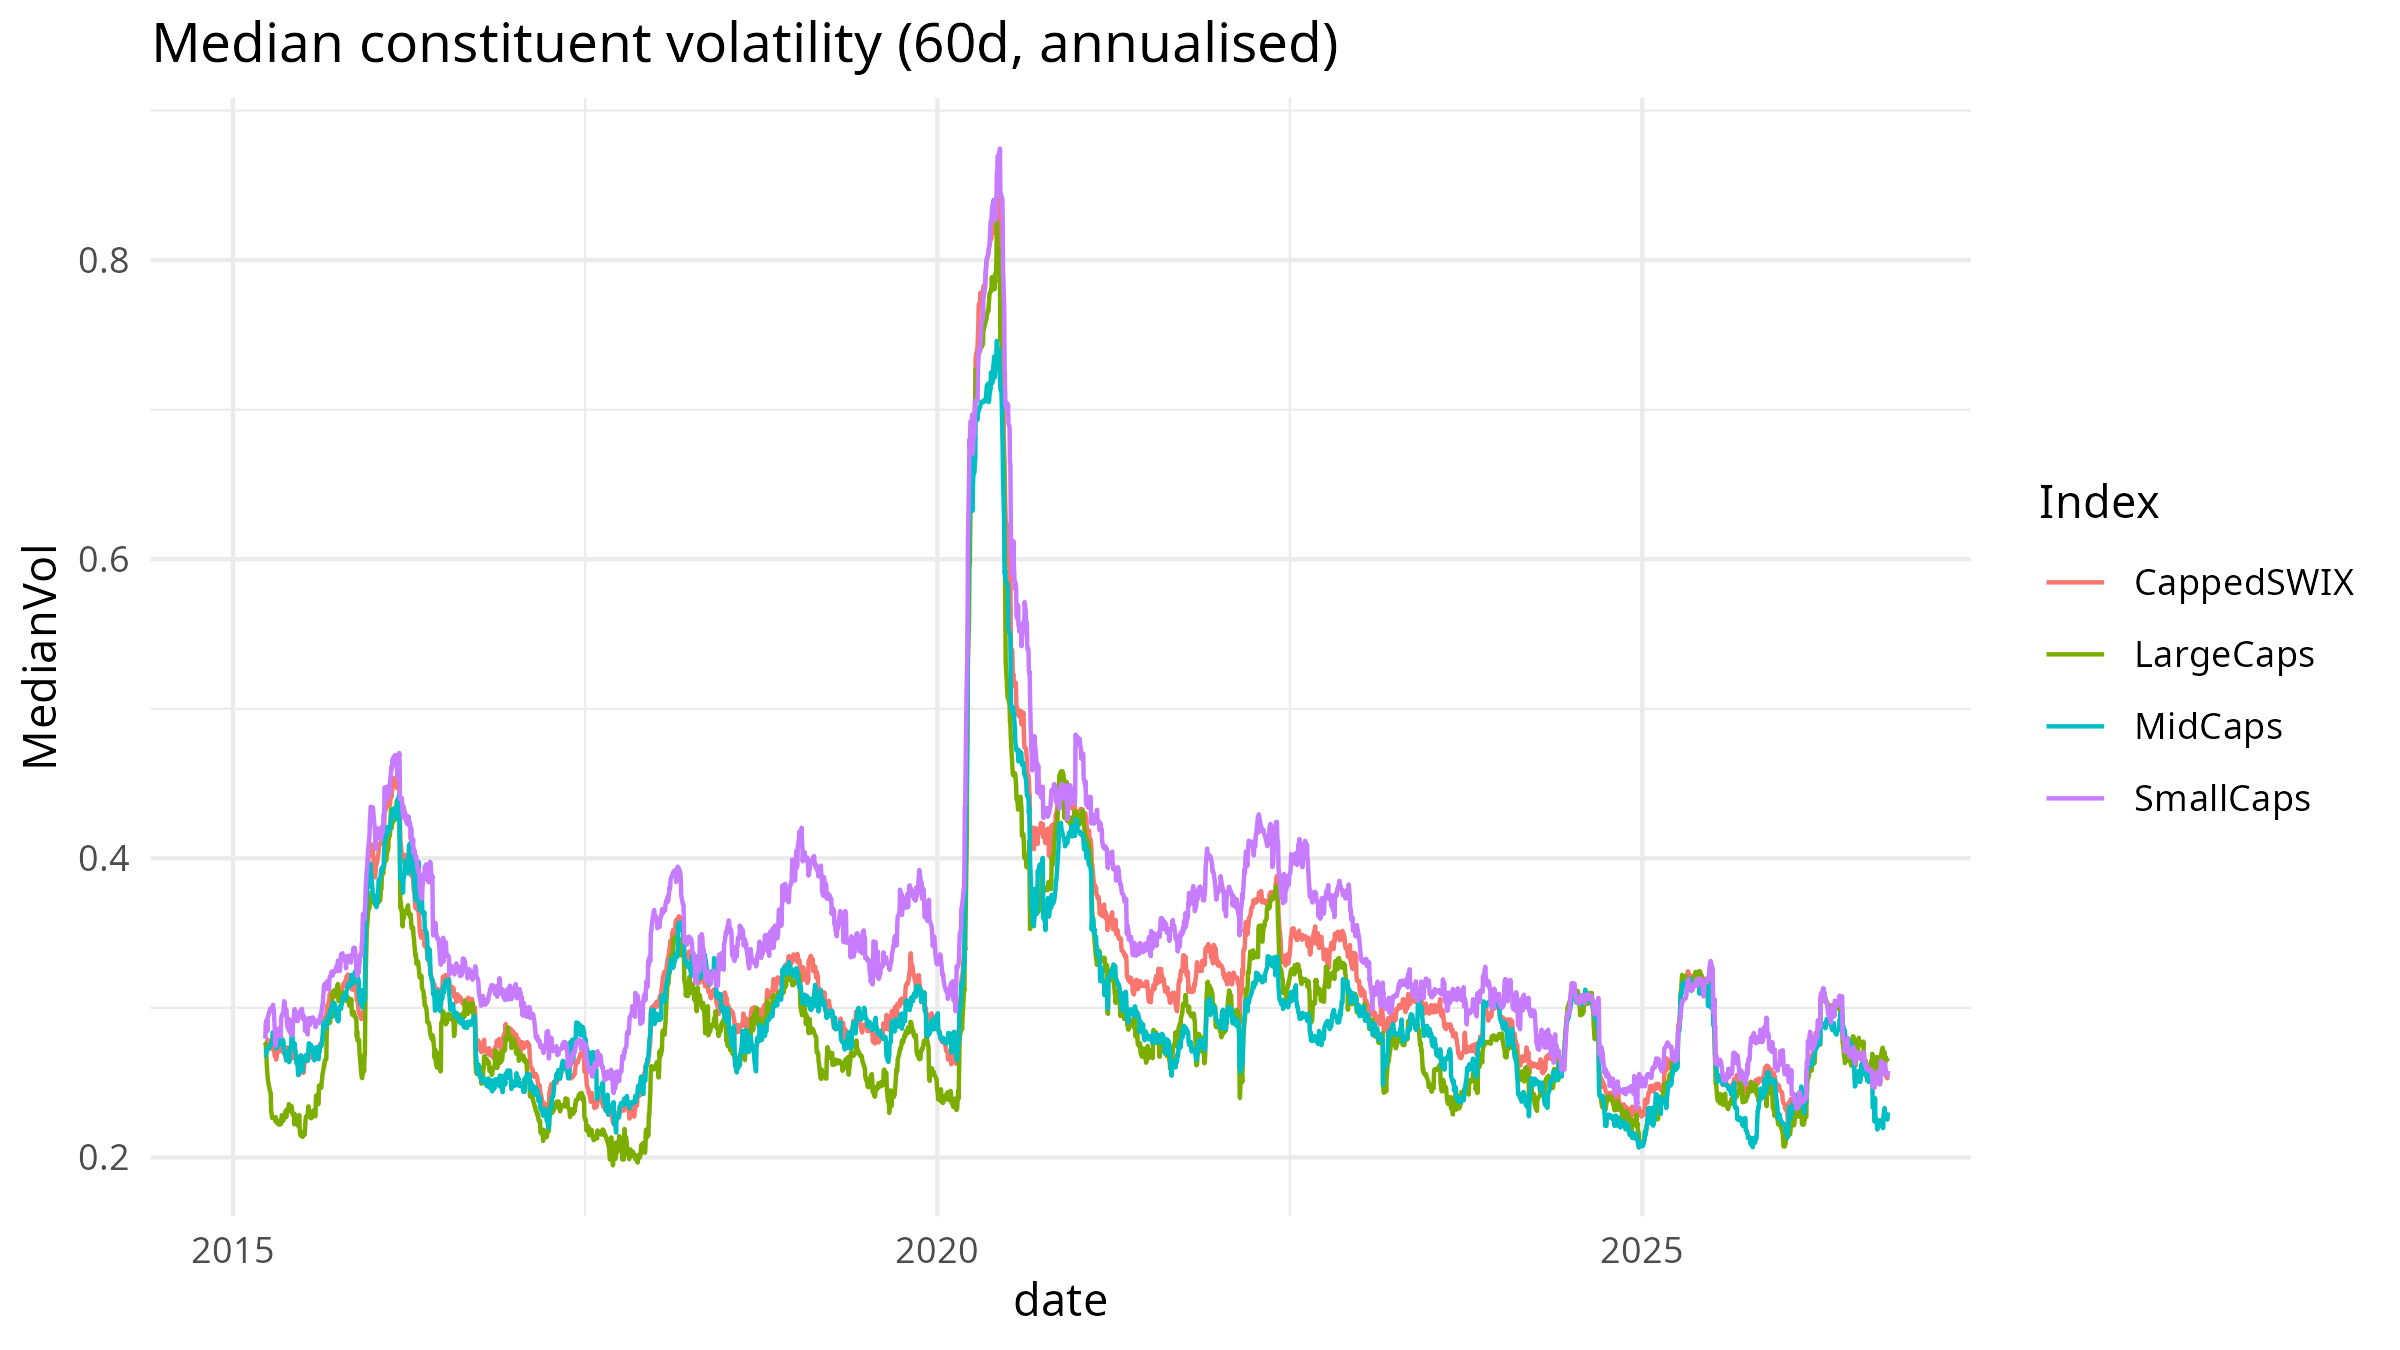
\includegraphics[width=1\linewidth]{../../figures/constituent_vol} \end{center}

The results in the table below shows the annualised stnadard deviationa
sn returns for periods of high, medium and low volatility. Where the the
high-vol regime corresponds to the times where the vol was in the top
third of its distribution , low-vol to bottom third and mid-vol to
middle.

\begin{longtable}[]{@{}llrr@{}}
\caption{Performance by volatility regime}\tabularnewline
\toprule\noalign{}
Index & Regime & AnnRet & AnnVol \\
\midrule\noalign{}
\endfirsthead
\toprule\noalign{}
Index & Regime & AnnRet & AnnVol \\
\midrule\noalign{}
\endhead
\bottomrule\noalign{}
\endlastfoot
CappedSWIX & Low vol & 0.349 & 12.053 \\
CappedSWIX & Mid vol & -5.130 & 15.082 \\
CappedSWIX & High vol & 34.943 & 23.546 \\
LargeCaps & Low vol & 2.287 & 13.267 \\
LargeCaps & Mid vol & -2.688 & 16.638 \\
LargeCaps & High vol & 36.747 & 24.517 \\
MidCaps & Low vol & 0.860 & 13.210 \\
MidCaps & Mid vol & -5.299 & 15.438 \\
MidCaps & High vol & 30.750 & 22.540 \\
SmallCaps & Low vol & 8.829 & 9.550 \\
SmallCaps & Mid vol & 8.912 & 11.474 \\
SmallCaps & High vol & 19.440 & 21.314 \\
\end{longtable}

\section{Index Return Profile}\label{index-return-profile}

Examining rolling annualised returns over 1-year and 3-year horizons
illustrates how return dispersion and cyclicality behave across JSE
market-capitalisation tiers: - High Short-Term Cyclicality (1Y): Over
1-year rolling windows, all four indices move largely in sync with broad
macroeconomic shocks, dropping into negative territory during the
early-2020 market sell-off before rebounding sharply. SmallCaps (purple)
exhibit the greatest upside amplitude, surging past 120\% during the
2021 recovery, whereas LargeCaps (green) and CappedSWIX (red) track
closely together with more moderated peaks. - Smoothed Long-Term
Trajectories (3Y): Extending the horizon to 3-year rolling periods
substantially dampens short-term noise, revealing a steady upward return
trend from 2020 onward. SmallCaps outperforms on a 3-year rolling basis
post-2021 until 2025 peaking near 50\% in early 2023---while MidCaps
(teal) frequently lag the broader benchmark over extended periods.

\begin{center}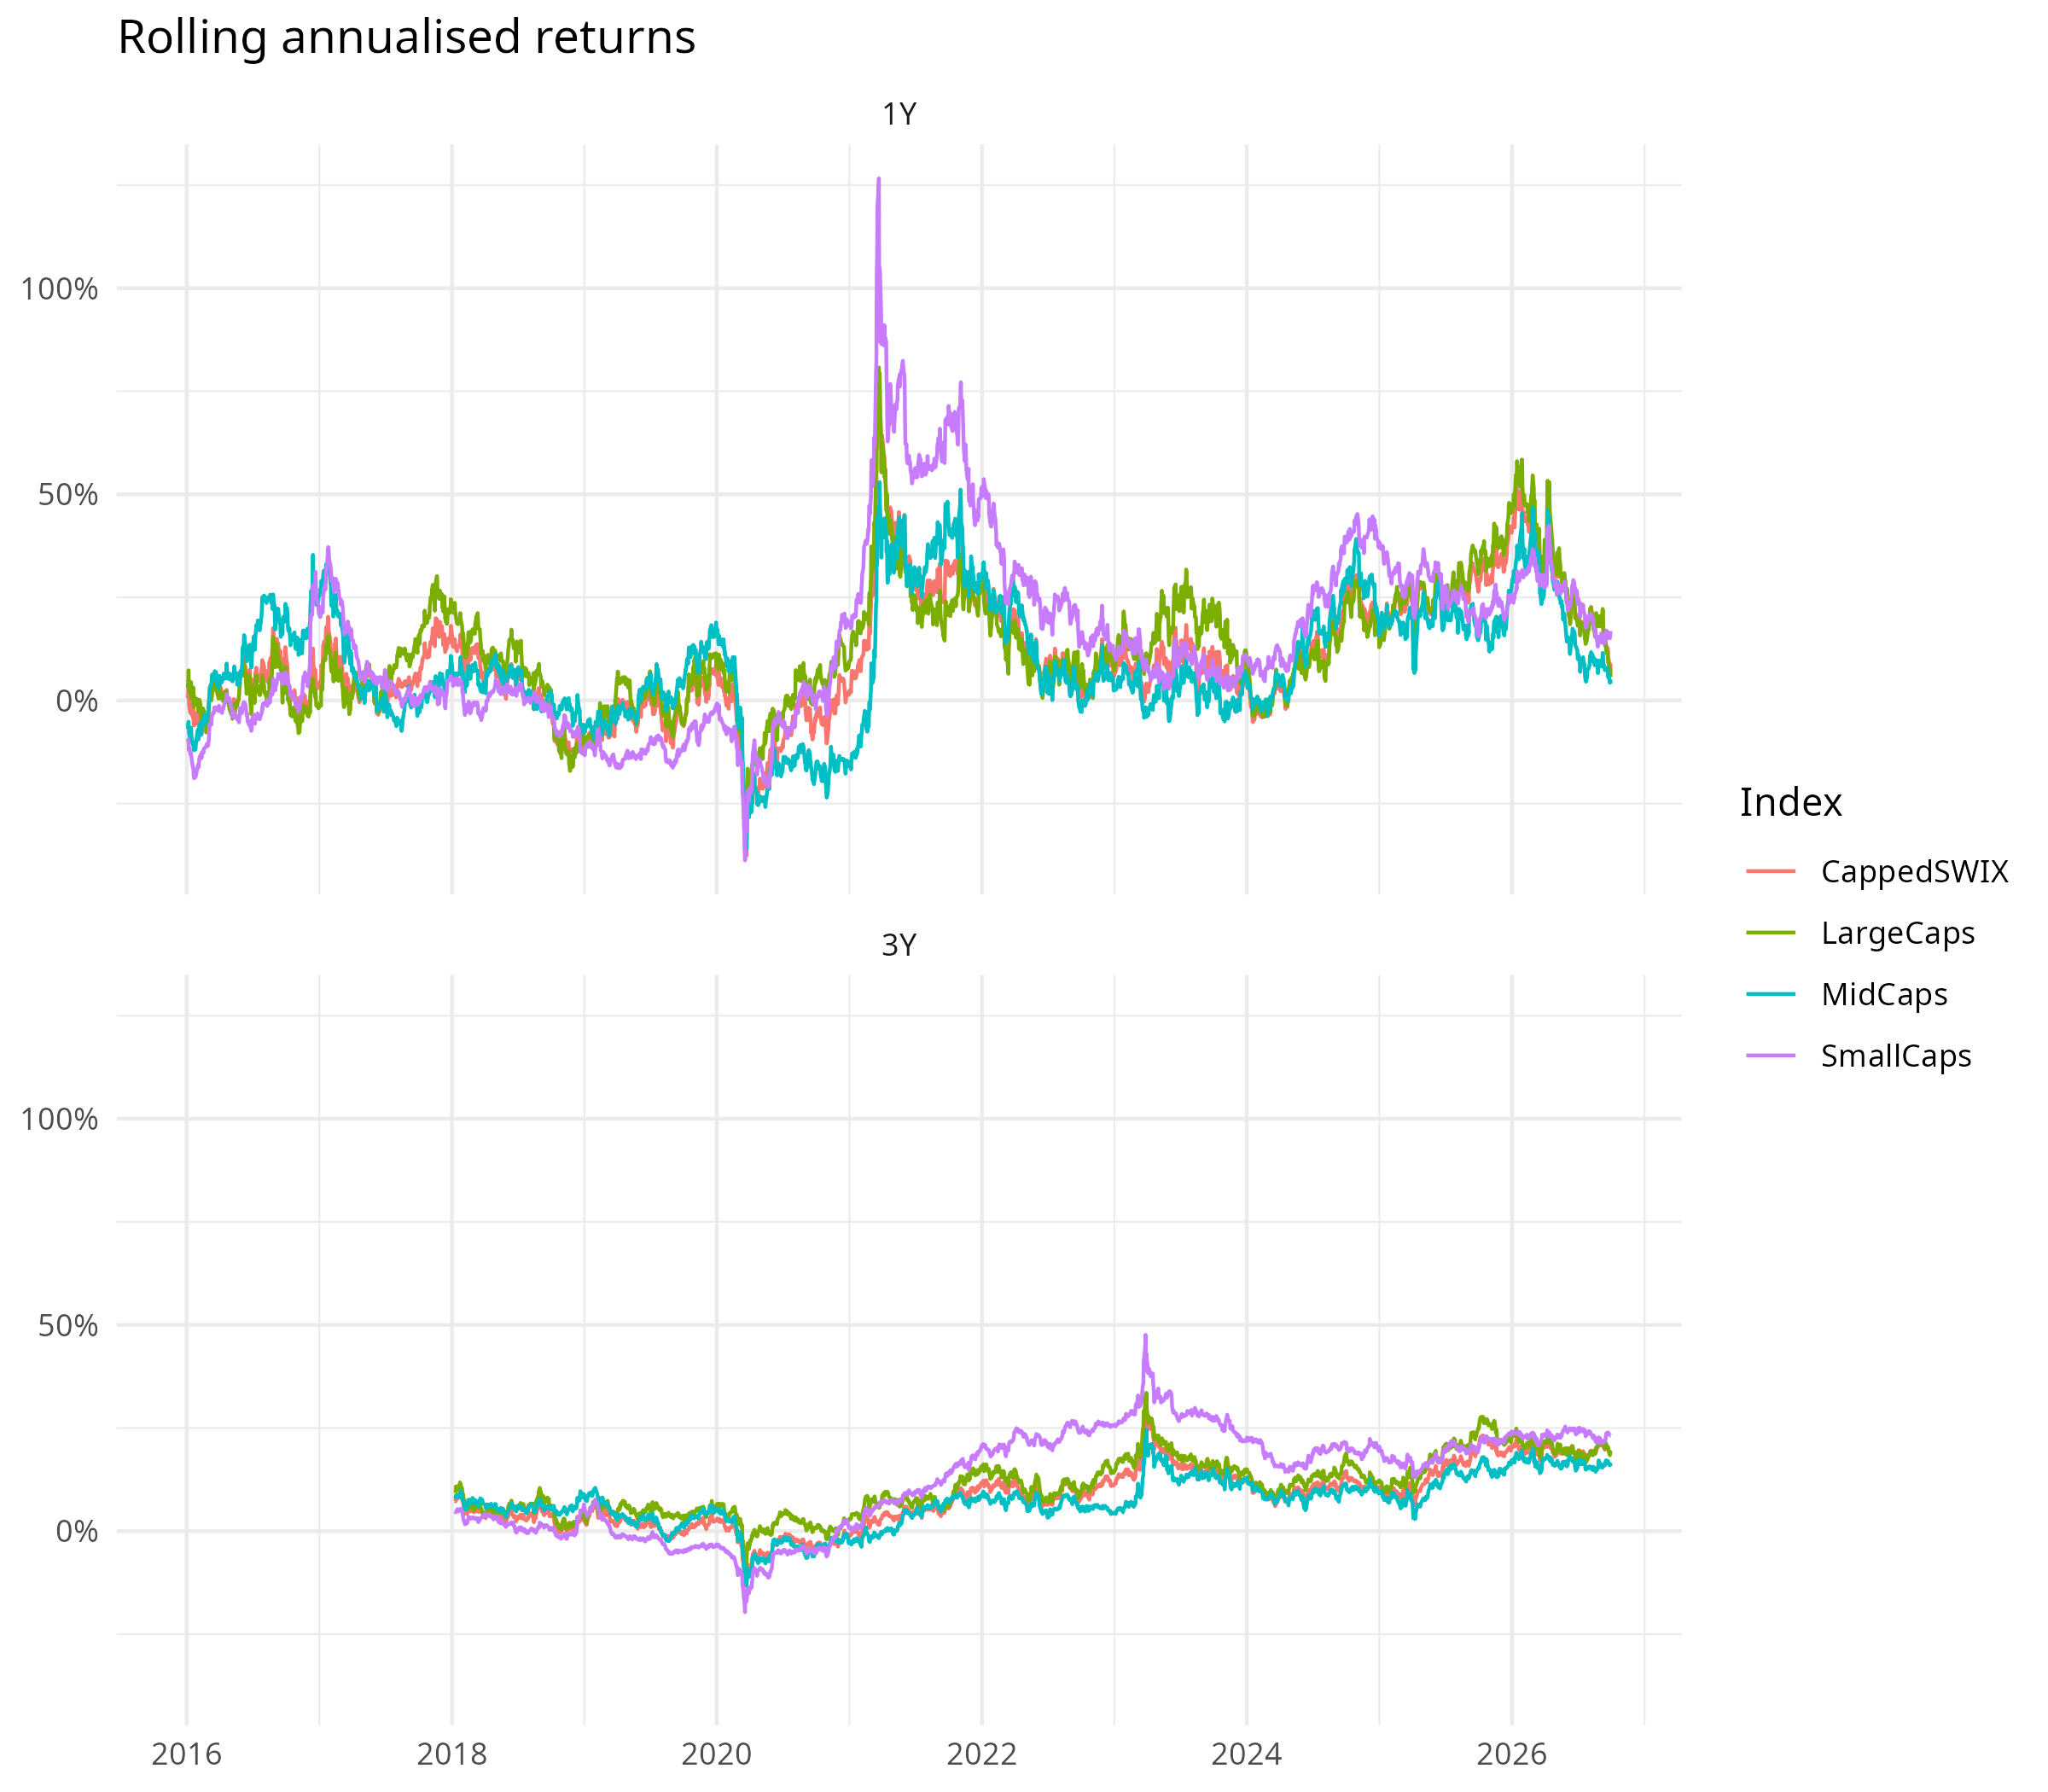
\includegraphics[width=1\linewidth]{../../figures/rolling_returns} \end{center}

\begin{longtable}[]{@{}lrrrr@{}}
\caption{Risk and return summary}\tabularnewline
\toprule\noalign{}
Index & AnnRet & AnnVol & RetPerRisk & MaxDD \\
\midrule\noalign{}
\endfirsthead
\toprule\noalign{}
Index & AnnRet & AnnVol & RetPerRisk & MaxDD \\
\midrule\noalign{}
\endhead
\bottomrule\noalign{}
\endlastfoot
CappedSWIX & 8.865 & 17.608 & 0.503 & -0.443 \\
LargeCaps & 10.898 & 18.768 & 0.581 & -0.385 \\
MidCaps & 7.486 & 17.541 & 0.427 & -0.426 \\
SmallCaps & 11.938 & 15.020 & 0.795 & -0.494 \\
\end{longtable}

\section{Index Active Share}\label{index-active-share}

Active share measures the percentage of a portfolio's holdings that
differ from the benchmark index, ranging from 0\% (an identical replica)
to 100\% (no overlapping holdings). Because the Capped SWIX is a
market-capitalisation-weighted benchmark dominated by large-cap
equities, active share increases dramatically as one moves down the size
spectrum:

\begin{center}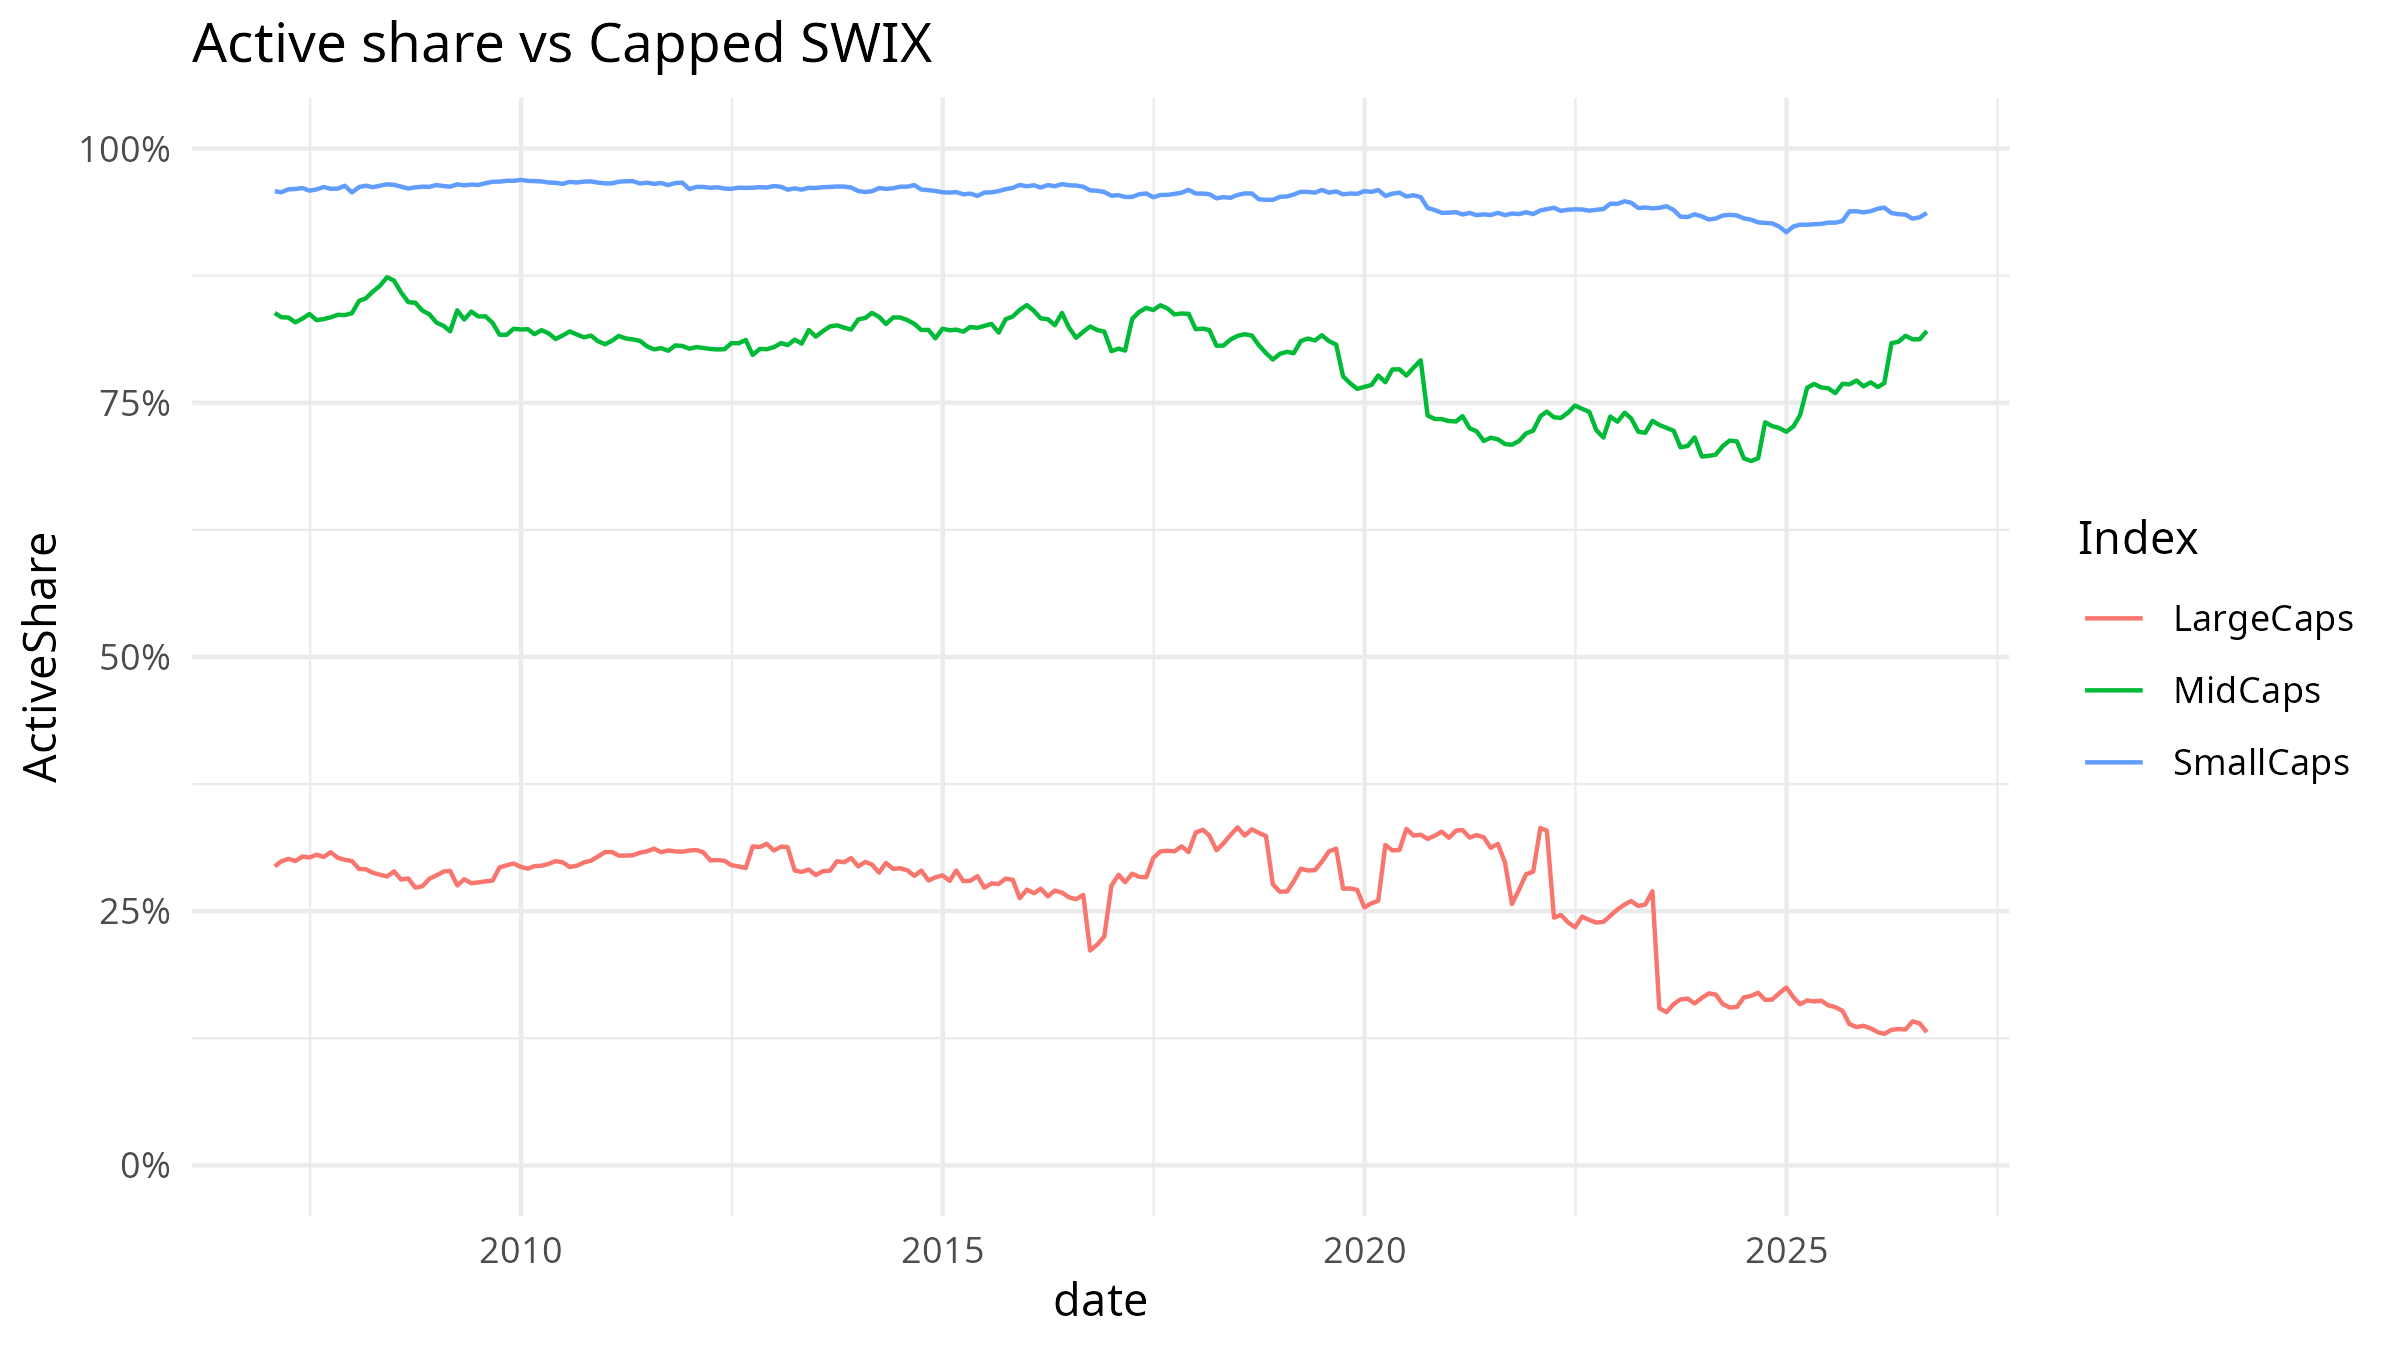
\includegraphics[width=1\linewidth]{../../figures/active_share} \end{center}

\begin{itemize}
\tightlist
\item
  LargeCaps (Mean: 26.8\%): Exhibit the lowest active share (ranging
  from 12.9\% to 33.2\%), reflecting substantial constituent overlap
  with the Capped SWIX. Notably, LargeCap active share dropped sharply
  after 2023---falling below 20\%---indicating an even tighter alignment
  with the benchmark's top holdings.
\item
  MidCaps (Mean: 79.4\%): Offer significant structural differentiation
  from the benchmark (ranging between 69.3\% and 87.3\%), though their
  active share trended gradually downward between 2017 and 2024 before
  rebounding toward 80\% recently.
\item
  SmallCaps (Mean: 95.3\%): Maintain a near-total divergence from the
  Capped SWIX across the entire sample period (ranging from 91.8\% to
  96.9\%), confirming that small-cap equities represent an almost
  entirely distinct opportunity set from the primary JSE benchmark.
\end{itemize}

\begin{longtable}[]{@{}lrrr@{}}
\caption{Active share versus the Capped SWIX}\tabularnewline
\toprule\noalign{}
Index & Mean & Min & Max \\
\midrule\noalign{}
\endfirsthead
\toprule\noalign{}
Index & Mean & Min & Max \\
\midrule\noalign{}
\endhead
\bottomrule\noalign{}
\endlastfoot
LargeCaps & 0.268 & 0.129 & 0.332 \\
MidCaps & 0.794 & 0.693 & 0.873 \\
SmallCaps & 0.953 & 0.918 & 0.969 \\
\end{longtable}

\section{Conclusion}\label{conclusion}

Comparing these South African Indices we again see that the market
compensates risk, as different indexes perfrom better in higher vol
regimes, SmallCaps outperforming during low- and mid-vol regimes.
Industrials are a major part of SOuth African indices and Financials
earning a larger share. Since 2020 SA indices apart from LargeCaps have
become less diversified.

\section{Appendix A}\label{appendix-a}

\begin{center}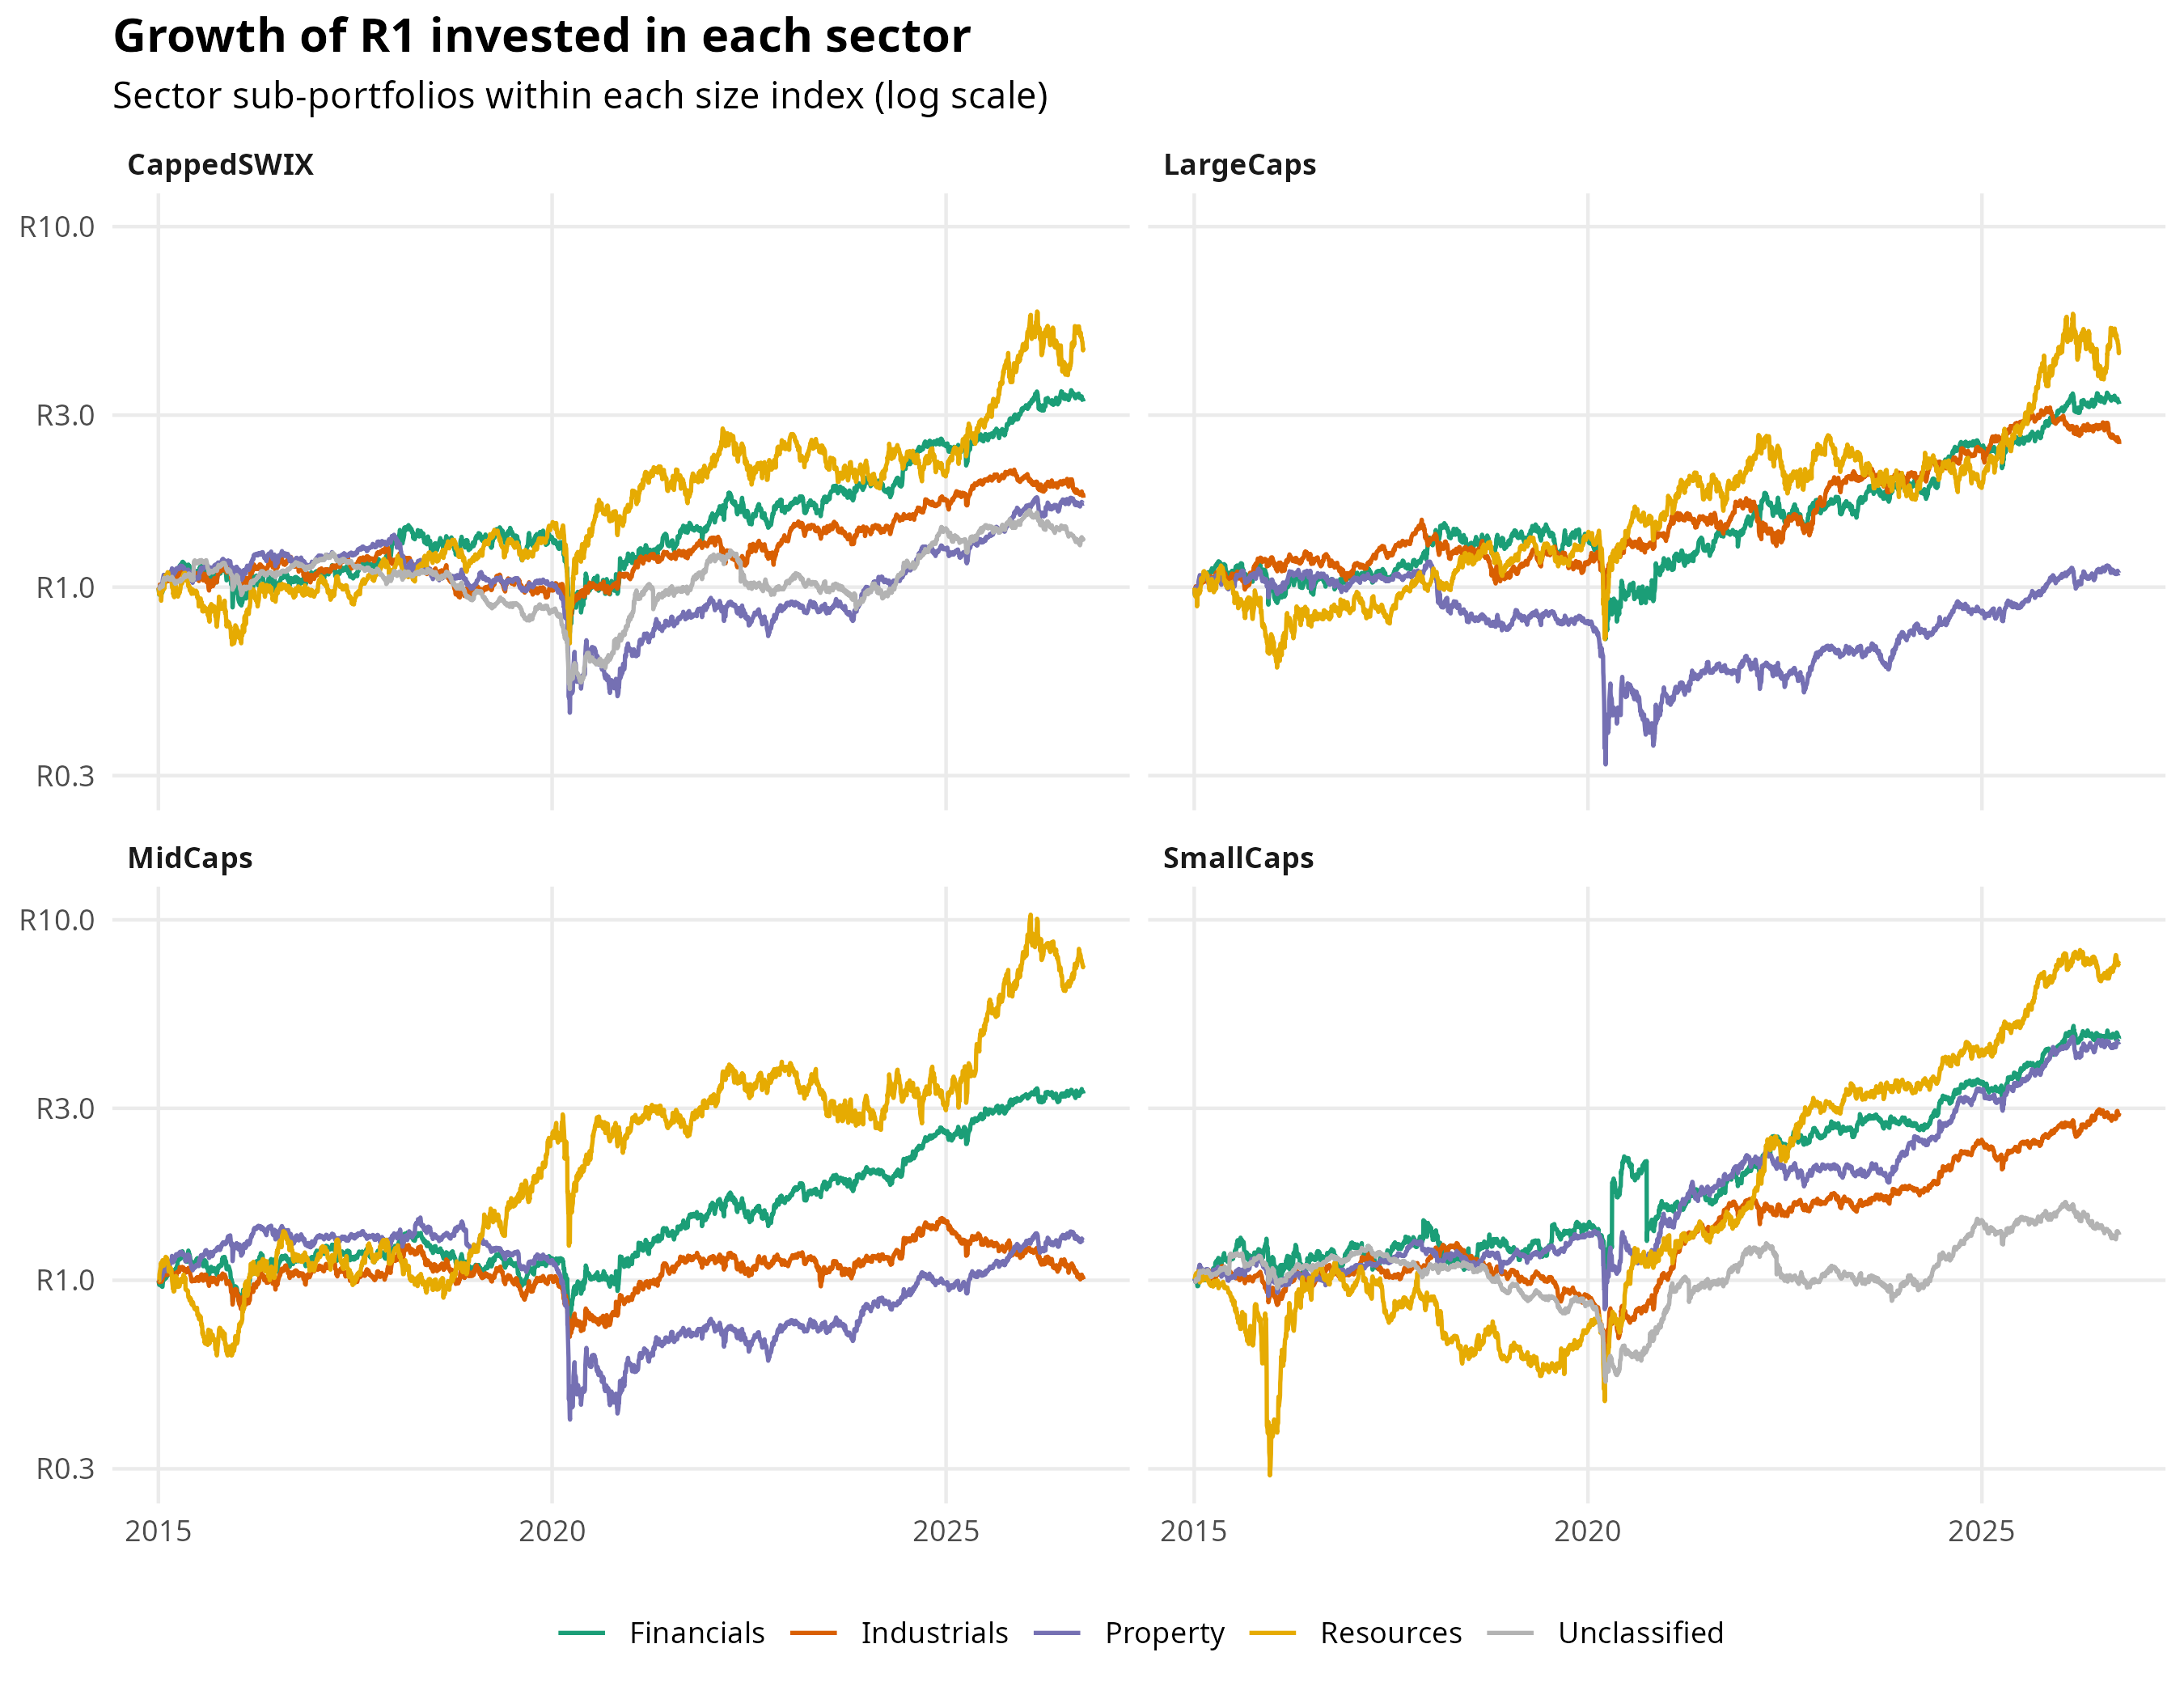
\includegraphics[width=1\linewidth]{../../figures/sector_growth} \end{center}

\begin{longtable}[t]{lrrrr}
\caption{\label{tab:ic_tab}Information criteria by model and index}\\
\toprule
Index & sGARCH & gjrGARCH & eGARCH & apARCH\\
\midrule
\addlinespace[0.3em]
\multicolumn{5}{l}{\textbf{Akaike}}\\
\hspace{1em}CappedSWIX & -6.395 & -6.417 & -6.420 & -6.407\\
\hspace{1em}LargeCaps & -6.218 & -6.243 & -6.249 & -6.234\\
\hspace{1em}MidCaps & -6.416 & -6.423 & -6.417 & -6.419\\
\hspace{1em}SmallCaps & -6.982 & -6.989 & -6.989 & -6.979\\
\addlinespace[0.3em]
\multicolumn{5}{l}{\textbf{Bayes}}\\
\hspace{1em}CappedSWIX & -6.384 & -6.404 & -6.408 & -6.393\\
\hspace{1em}LargeCaps & -6.208 & -6.231 & -6.236 & -6.220\\
\hspace{1em}MidCaps & -6.406 & -6.411 & -6.405 & -6.404\\
\hspace{1em}SmallCaps & -6.972 & -6.977 & -6.976 & -6.964\\
\bottomrule
\end{longtable}

\begin{center}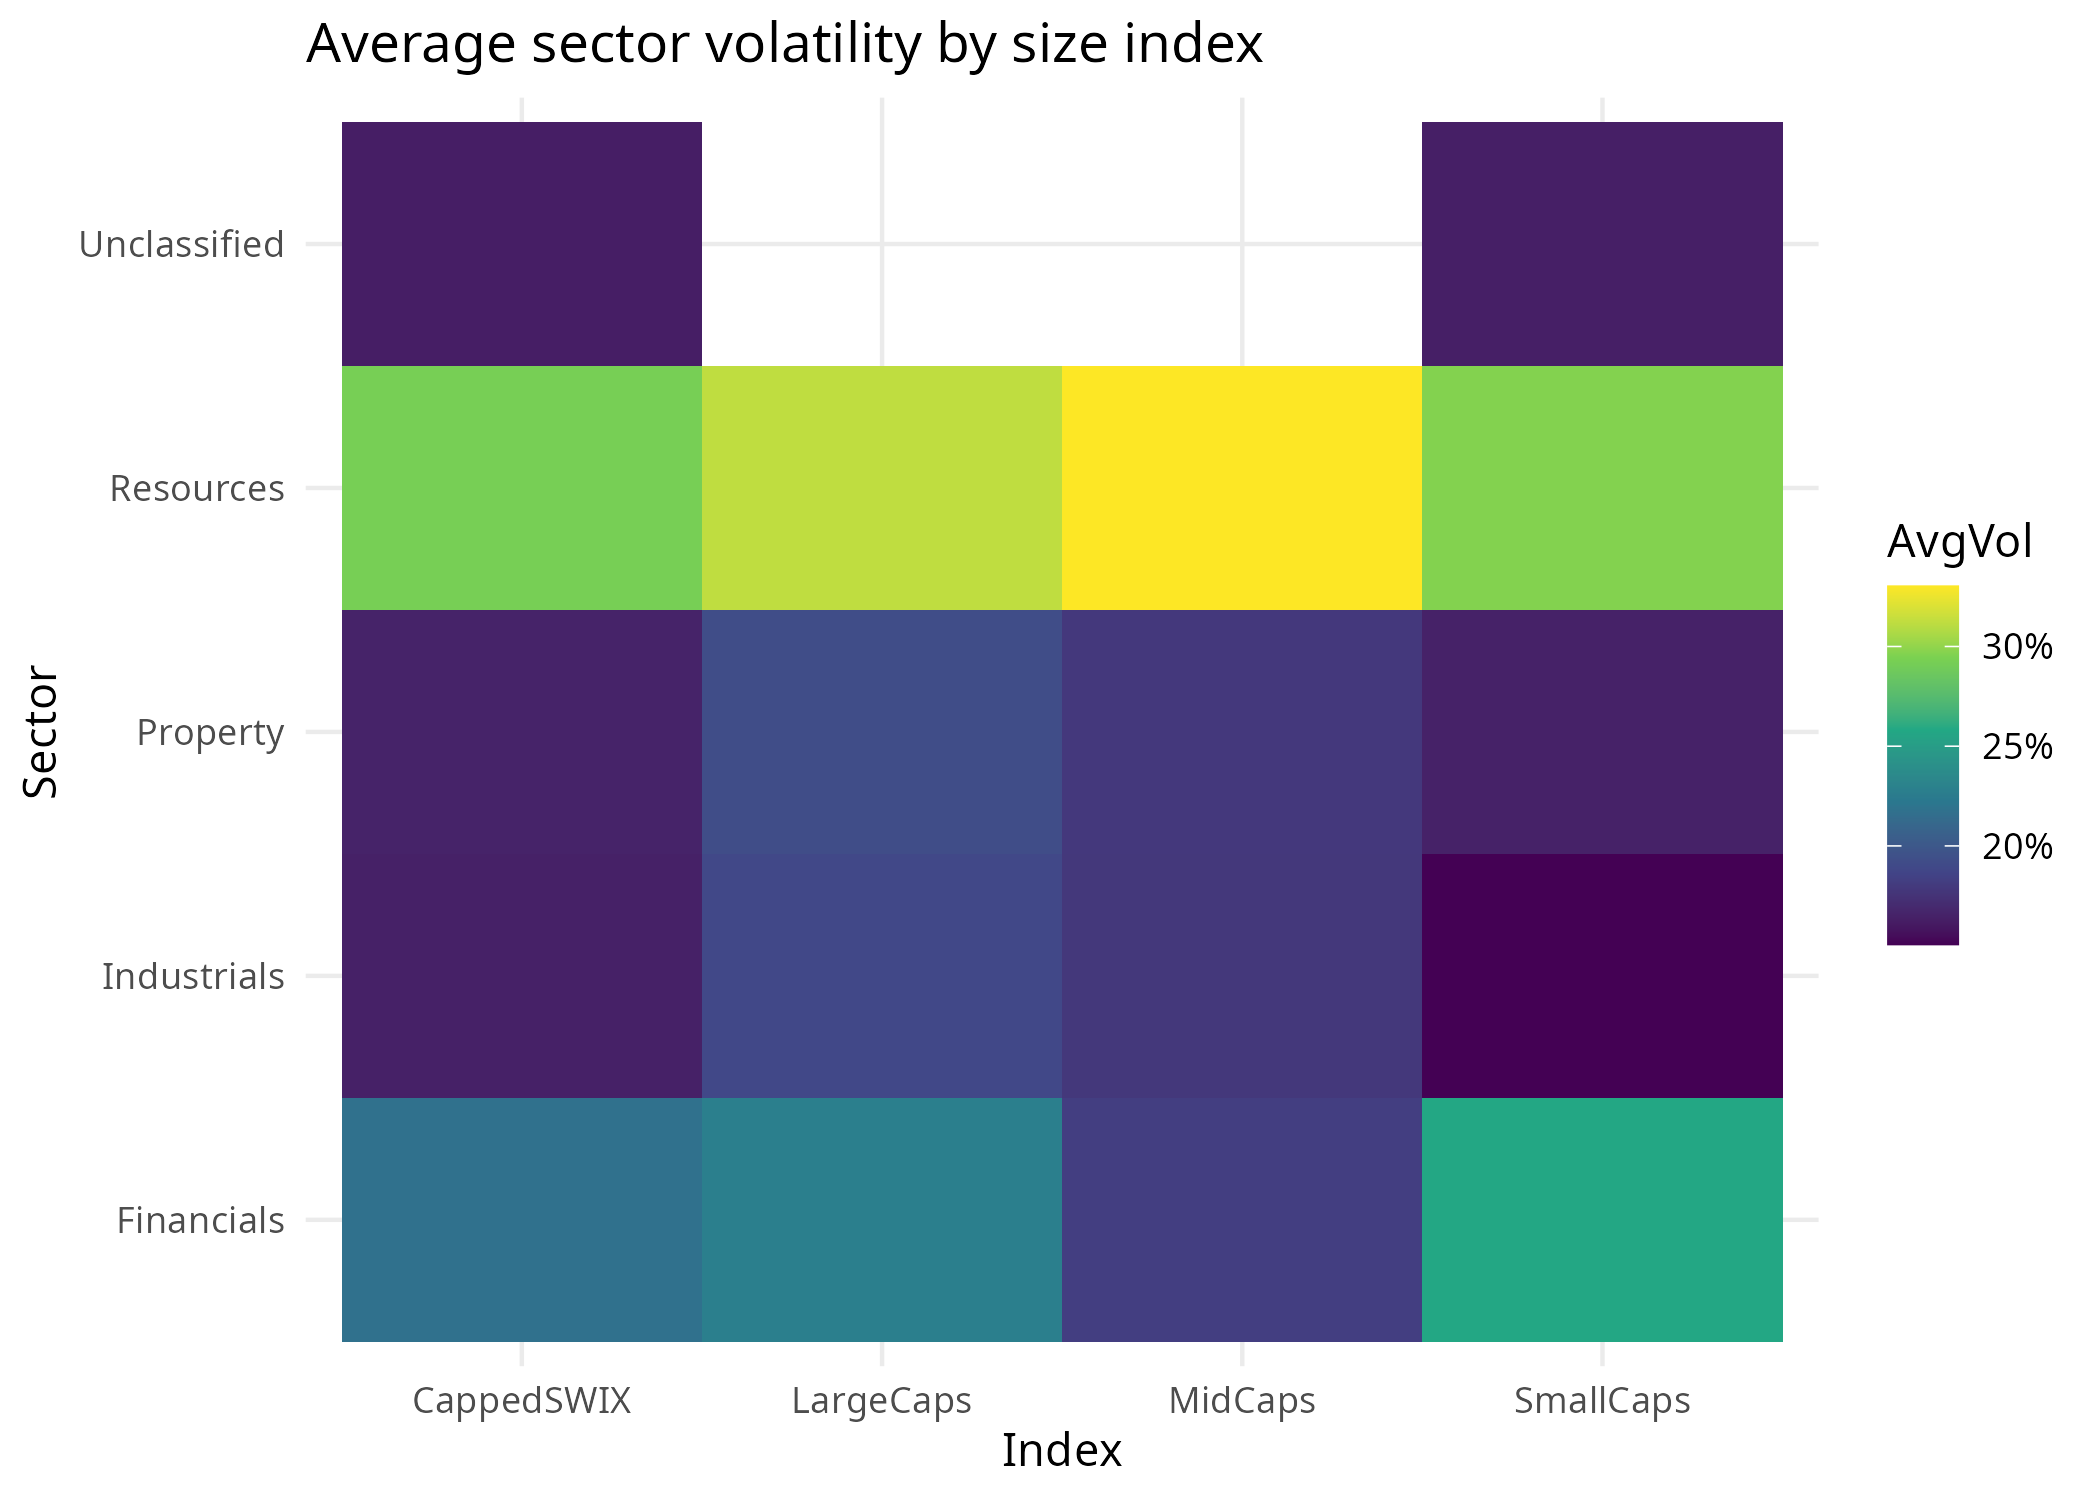
\includegraphics[width=1\linewidth]{../../figures/sector_vol_heat} \end{center}

\bibliography{Tex/ref}





\end{document}
